\documentclass[openany]{book}
\input{notes_white}
\usepackage{mathtools}
\usepackage{pgfplots}
\settitle{Probability and Stats 1  Notes and Solutions}
\begin{document}
\title{\Large{\underemphasise{Probability and Statistics Notes}} \\ \vspace{5pt}
\large{Prob Stats 1: Notes, Exercises and PYQs}}
\author{Eklavya Raman \\ \vspace{5pt} er24ms024@iiserkol.ac.in \\ \vspace{5pt}}
\date{\today}
\maketitle
\tableofcontents
\listoftheorems[
    show=mytheorem,
    title={List of Theorems}]

\part{Probability}
\chapter{Continous Random Variables and Distributions}
\section{Continous Random Variables}
Let us first define what a continous function and a continous random variable is.
\begin{mydefinition}{Continous Function}
    A function \( f: \mathbb{R} \to \mathbb{R} \) is said to be continous at a point \( x_0 \in \mathbb{R} \) if for every \( \epsilon > 0 \), there exists a \( \delta > 0 \) such that for all \( x \in \mathbb{R} \), if \( |x - x_0| < \delta \), then \( |f(x) - f(x_0)| < \epsilon \). If a function is continous at every point in its domain, it is called a continous function.
\end{mydefinition}
Let us consider a simple example of a continous function ($f(x) = \sin (x)$) - 
\begin{figure}[H]
    \centering
    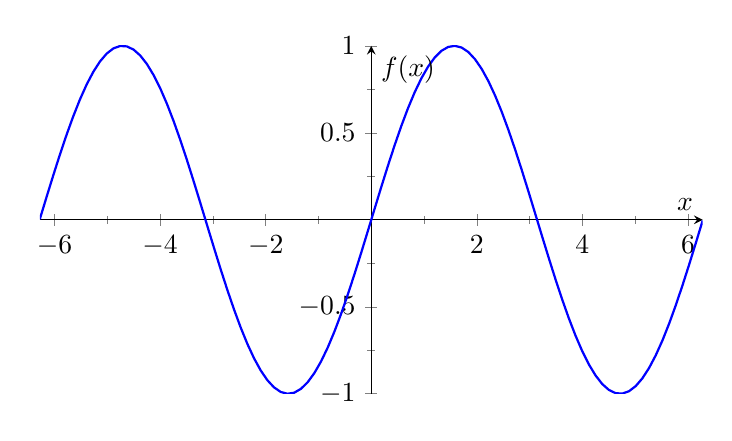
\begin{tikzpicture}
        \begin{axis}[
            axis lines = middle,
            xlabel = \( x \),
            ylabel = {\( f(x) \)},
            domain= -6.28:6.28,
            samples=100,
            width=10cm,
            height=6cm,
            grid=none,
            minor tick num=1,
        ]
        \addplot [blue, thick] {sin(deg(x))};
        \end{axis}
    \end{tikzpicture}
    \caption{Graph of the continous function \( f(x) = \sin(x) \)}
\end{figure}
\begin{mydefinition}{Continous Random Variable}
    A random variable \( X \) is said to be continous if its cumulative distribution function (CDF) \( F_X(x) = P(X \leq x) \) is continous for all \( x \in \mathbb{R} \).
\end{mydefinition}
Now, we define the probability density function (PDF) for a continous random variable.
\begin{mydefinition}{Probability Density Function (PDF)}
    The probability density function (PDF) of a continous random variable \( X \) is a function \( f_X(x) \) such that for any two numbers \( a \) and \( b \) with \( a < b \),
    \[
        P(a < X < b) = \int_{a}^{b} f_X(x) \, dx
    \]
    The PDF must satisfy the following properties:
    \begin{enumerate}
        \item \( f_X(x) \geq 0 \) for all \( x \in \mathbb{R} \)
        \item \( \int_{-\infty}^{\infty} f_X(x) \, dx = 1 \)
    \end{enumerate}
\end{mydefinition}
We also now define the cumulative distribution function (CDF) for a continous random variable.
\begin{mydefinition}{Cumulative Distribution Function (CDF)}
    The cumulative distribution function (CDF) of a continous random variable \( X \) is a function \( F_X(x) \) defined as
    \[
        F_X(x) = P(X \leq x) = \int_{-\infty}^{x} f_X(t) \, dt
    \]
    where \( f_X(t) \) is the probability density function (PDF) of \( X \).
\end{mydefinition}
Now, we are equipped to study these continous random variables and their distributions in detail. \\\\
Let $X \sim f(x) \nd F(x)$, let $Y = g(X)$, where g is strictly monotonic and differentiable. Then, 
$$F_Y(y) = P(Y \leq y) = P(g(X) \leq y) = \begin{dcases}
    P(X \leq g^{-1}(y)), & \text{if g is increasing} \\
    P(X \geq g^{-1}(y)), & \text{if g is decreasing}
\end{dcases}$$
We also have - 
$$f_Y(y) = \begin{dcases}
    f(g^{-1}(y)) \cdot \frac{d}{dy} g^{-1}(y), & \text{if g is increasing} \\
    f(g^{-1}(y)) \cdot \left| \frac{d}{dy} g^{-1}(y) \right|, & \text{if g is decreasing}
\end{dcases}$$
Therefore, we can simply write - 
$$f_Y(y) = f(g^{-1}(y)) \cdot \left| \frac{d}{dy} g^{-1}(y) \right| \sim f(x) \cdot |\frac{dx}{dy}|$$
Now, let us consider the case where $g$ is monotone, but not strictly monotone. This means that there exists an interval where $g$ is constant. Let us denote this interval as $[a, b]$. In this case, for any $y$ in the range of $g$ corresponding to the interval $[a, b]$, we have -
$$P(Y = y) = P(g(X) = y) = P(X \in [a, b]) = \int_{a}^{b} f_X(x) \, dx$$
Let $g^{-1}(y) = \inf \{x: g(x \geq y) \}$, then we have -
$$F_Y(y) = P(Y \leq y) = P(g(X) \leq y) = P(X \leq g^{-1}(y)) = F_X(g^{-1}(y))$$
Differentiating both sides with respect to $y$, we get -
$$f_Y(y) = f_X(g^{-1}(y)) \cdot \frac{d}{dy} g^{-1}(y)$$
However, since $g$ is not strictly monotone, we need to account for the intervals
where $g$ is constant. Therefore, we can write the PDF of $Y$ as -
$$f_Y(y) = f_X(g^{-1}(y)) \cdot \left| \frac{d}{dy} g^{-1}(y) \right| + \sum_{i} P(X \in [a_i, b_i]) \cdot \delta(y - g(c_i))$$
where $[a_i, b_i]$ are the intervals where $g$ is constant, $c_i$ is any point in the interval $[a_i, b_i]$, and $\delta$ is the Dirac delta function. This accounts for the probability mass at the points where $g$ is constant. \\\\
\subsubsection{Example}
Let $X \sim f(x) = \begin{dcases}
    \frac{1}{2}, & -0.5 \leq x \leq 1.5 \\
    0, & \text{otherwise}
    \end{dcases}$ 
    and $Y = X^2$. We need to find the distribution of $Y$. \\\\
We have -
$$F_Y(y) = P(Y \leq y) = P(X^2 \leq y) = P(-\sqrt{y} \leq X \leq \sqrt{y})$$
Therefore,
$$F_Y(y) = \int_{-\sqrt{y}}^{\sqrt{y}} f_X(x) \, dx = \int_{-\sqrt{y}}^{\sqrt{y}} \frac{1}{2} \, dx = \frac{\sqrt{y} - (-\sqrt{y})}{2} = \sqrt{y}$$
for $0 \leq y \leq 2.25$. Differentiating, we get -
$$f_Y(y) = \frac{d}{dy} F_Y(y) = \frac{1}{2\sqrt{y}}$$
for $0 < y \leq 2.25$. Thus, the distribution of $Y$ is given by -
$$f_Y(y) = \begin{dcases}
    \frac{1}{2\sqrt{y}}, & 0 < y \leq 2.25 \\
    0, & \text{otherwise}
\end{dcases}$$



\end{document}